The two major categories of cartography are general cartography and thematic cartography, which are introduced in chapter \ref{s:cartography} on page \pageref{s:cartography}. This categorization can be directly adopted from cartography to maps. The main objective of this chapter is to give an overview of different thematic maps and their usage. These maps can be subdivided into univariate and multivariate maps.

\paragraph{Univariate Thematic Map Types}
\label{s:univariate-maps}

Univariate maps are only dependent on one variable, except for the map variables like latitude and longitude. This section contains four different univariate maps and is going to explain them in detail.

\subparagraph{Dot density map}
\label{s:dot}
The first dot map in history is shown in figure \ref{fig:cholera-map} on page \pageref{fig:cholera-map}. It was the first map of its kind and could help in the display of disease outbreaks. This type of univariate thematic map uses points or dots to map discrete data. Attribute values of the given data determine the number of dots displayed in a specific regions. All dots need to be the same size. To explain the two different types of dot maps, imagine a dataset of customers where each customer has a location:

\begin{enumerate}
\ditem{One-to-one} \hfill \\
Each dot on the map represents exactly one item of the represented theme. Considering the example dataset mentioned above, every customer would be represented by exactly one dot.
\ditem{One-to-many} \hfill \\
Each dot on the map represents an aggregate of information. Therefore this type of dot map could be used with the aggregation of customers in a specific location. Thus the map maker needs to make the decision how many customers are aggregated, or rather how many customers are represented by one dot.
\end{enumerate}

Both types of dot density maps share the purpose, that they are not a tool to determine exact quantities. Getting the exact amount of dots in a high density area is a very cumbersome task and users often tend to underestimate dot totals as density increases \iacite{McMaster2001}. However, it is a very common technique for viewing the clustering, dispersion, linearity, and general pattern of a distribution. The technique appeared first in the 19\textsuperscript{th} century and is today accepted as one of the primary techniques for representing geographic patterns \iacite{Tyner2010}.

The map maker can use dots in a dot density map with a different type of level of detail. This means, that dots do not necessarily need to have an exact location. If he or she wants to discover a pattern on a state-wide level of detail, dots can be placed anywhere in their corresponding states, as long as they do not leave their state boundaries.
Another location based decision the map maker needs to make is, if the dots should use some kind of pseudo-random placement in case of overlapping. This decision is based on a maximum overlap constraint. It can be thought of as a random placement of dots in a square without violating the constraint.

According to \citeauthor{Tyner2010}, there are some main design principles for dot maps that should be considered:
\begin{itemize}
\item The size of the dot.
\item The value assigned to the dot. This also includes the correct use of the two different types of dot maps.
\item The location of the dot on the map in case of an aggregated level of detail of the map.
\item The aggregated units in case of a one-to-many dot map. This design principle can be thought of as using a legend in order to tell the aggregated value one dot represents.
\end{itemize}
Changing any one of these can change the overall appearance and interpretation of the map \iacite{Tyner2010}.

The main advantage of this type of map is the understandability. It requires little to no cognitive effort by the user to read the map when compared to other types. Specific advantages of dot maps are the good measure of density and the loose coupling between the size of a dot and its represented value.
However, reading specific information from those maps is not an easy task as mentioned before. Additionally, if a map uses some kind of random placement without any hint in the visualization, map readers may potentially infer the locations of dots as precise locations of the mapped phenomenon. To counteract the second drawback, dot density maps with random placement of dots should consider the acual occurence of the mapped phenomenon, e.g. dots should not be placed in lakes for a map of population.

\subparagraph{Graduated symbol or proportional symbol map}
Figure \ref{fig:first-mixture} on page \pageref{fig:first-mixture} shows a special kind of a proportional symbol map. According to figure \ref{fig:va-channels} on page \pageref{fig:va-channels}, this type of map uses the visual channel of size to represent differences of discrete data. Again, this type of map can be subdivided into two categories: classed and unclassed. Classed ones are known as range-graded or graduated symbol maps, whereas unclassed ones are called proportional symbol maps. The latter one uses a symbol size proportional to the value of the attribute being mapped \iacite{Dutton.2014}.
Although circles are the most typical symbol used, it is possible to use any type of symbol, ranging from abstract, geometric symbols to pictographic symbols. Figure \ref{fig:different-symbols} on page \pageref{fig:different-symbols} shows two proportional symbol maps showing the same phenomenon. The left part of this figure uses the common circle as symbol, while the right side uses a pictogram. Albeit, \citeauthor{Dutton.2014} says, that squares or bars are easier to estimate the size of the symbol. However, the circle established because of its compactness due to its low perimeter to area ratio.

\begin{figure}[!htb]
\centering
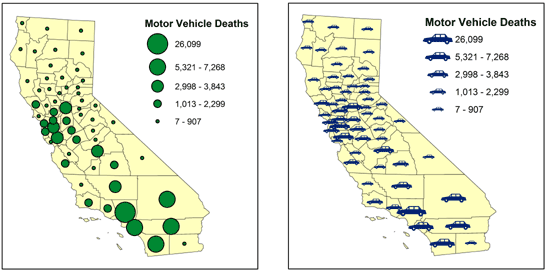
\includegraphics[height=5cm,keepaspectratio]{images/psm/symbols.png}
\caption[
    Two types of proportional symbol maps with different symbols \iacite{Dutton.2014}.
]{Two types of proportional symbol maps with different symbols.}
\label{fig:different-symbols}
\end{figure}

Another consideration in terms of symbol used is the fact, that squares and bars tend to run off the page with large values earlier than circles might \iacite{Dutton.2014}. \citeauthor{FLANNERY1971} introduced a scaling factor for proportional circles for better estimation of the value. However, this correction may not be very effective, because the correction itself does not consider the map context \iacite{FLANNERY1971}. A phenomenon related to the importance of context is known as the Ebbinghaus illusion. Figure \ref{fig:ebbinghaus} on page \pageref{fig:ebbinghaus} shows such an illusion. Both central circles actually have the same size, but because of the context of each side, the central circles appear different.

\begin{figure}[!htb]
\centering
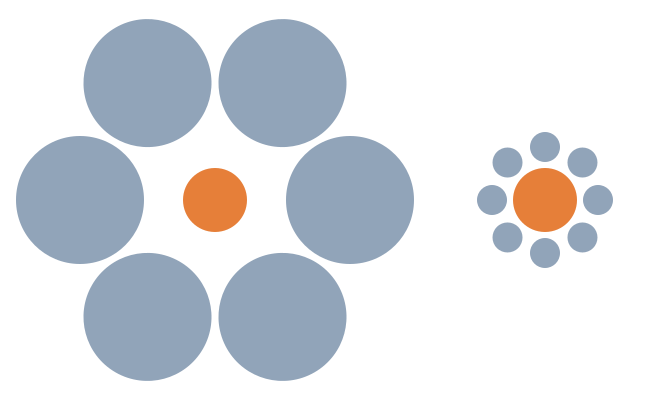
\includegraphics[height=5cm,keepaspectratio]{images/psm/ebbinghaus.png}
\caption[
    Ebbinghaus illusion, Urldate: 07.2016 \newline
    \small\texttt{\url{https://upload.wikimedia.org/wikipedia/commons/b/bc/Mond-vergleich.svg}}
]{Ebbinghaus illusion}
\label{fig:ebbinghaus}
\end{figure}

In order to combat the problem of value estimation, there are two major choices:
\begin{enumerate}
\item A legend could show proportional symbols which represent the different values of the mapped phenomenon. One possibility would be to display the smallest symbol, the largest symbol and some symbols at intermediate values.
\item Another alternative is to use range-graded symbols. Therefore the data needs to be classified, but in exchange the estimation problem is completly avoided. This alternative still needs consideration in the size of symbols, because each symbol should still be distinguishable from each other.
\end{enumerate}

Based on the given knowledge about proportional and gradient symbol maps, it is possible to derive some main design principles:
\begin{itemize}
\item The estimation of the value of a symbol is key for this type of map. This is most easily accomplished with geometric symbols.
\item Use a legend with examples to increase the reader's ability to correctly estimate the value of a symbol.
\end{itemize}

A close related problem to the user's estimation problem is the actual scaling technique used. According to \citeauthor{Dent2008} the three most commong techniques used are
\begin{enumerate*}
\item absolute scaling,
\item apparent magnitude scaling and
\item range grading \iacite{Dent2008}.
\end{enumerate*}

\begin{enumerate}
\ditem{Absolute scaling} makes each symbol fit its data value on the scale being used. This means, that a symbol representing four items in a dataset is twice as big as a symbol representing two.
\ditem{Apparent magnitude scaling} compensates for human error interpretation in scale. Using this technique, a symbol having twice as much in value is not twice as big, because it would appear smaller, leading to interpretation error. This type of scaling takes this error into account and increased the size of a symbol by more than the proportional amount \iacite{Krygier.2007}.
\ditem{Range grading} classifies the data into a fixed amount of groups. Each group has a fixed range of values and the same symbol to represent. The groups only differ in the range of values they represent and the size of the symbols.
\end{enumerate}

The main advantage of a proportional symbol map is the flexibility it comes along with. Possible data can either be numerical or categorical nature. Even the way the data is used is adjustable. An item can be mapped on a precise location or to geographic areas, depending on the level of detail.
Comparing proportional symbol maps with dot density maps, one advantage is observable: the estimation problem of dot density maps becomes less tedious when using proportional symbols. However, if proportional symbol maps are put in comparison with choropleth maps, they also have an advantage: the size of the enumeration unit does not matter. This problem will be explained in detail in chapter \ref{s:choropleth} on page \pageref{s:choropleth}.

\subparagraph{Choropleth map}
For continuous data, two mapping techniques are commonly used: choropleth and isarithmic mapping. This chapter will only cover choropleth mapping because the practical part of this thesis will not feature isarithmic mapping. The basic idea of choropleth mapping is applying value or color intensity based on some statistical value to enumeration units like census tracts, counties, states or nations. The higher a value assigned to an enumeration unit, the more saturated the color of that unit. Fundamental to this type of mapping is standardization and classification of raw data. If this is not the case and raw data is used, the visualization will suffer from an inherent areal bias \iacite{McMaster2010}. This problem is best described with a practical example: the united kingdom has higher population but less area compared to canada. However, if the mapped data is not standardized by area, canada will have a higher visual impact than united kingdom due to their superior areal extent, even though the attribute mapped onto canada has a lower value compared to the one on united kingdom. Therefore the less the mapped attribute is tied to enumeration units, the less sense a choropleth map makes.

The following list shows the most rudimentary and most common methods to classify data mentioned by \citeauthor{McMaster2010}. The amount of classes must be known before and to explain the classifications below, five different classes with a value range from 10 to 85 is used. Figure \ref{fig:choropleth-classification} on page \pageref{fig:choropleth-classification} illustrates an example showing all values as circles on the top and their corresponding classification downwards.

\begin{figure}[!htb]
\centering
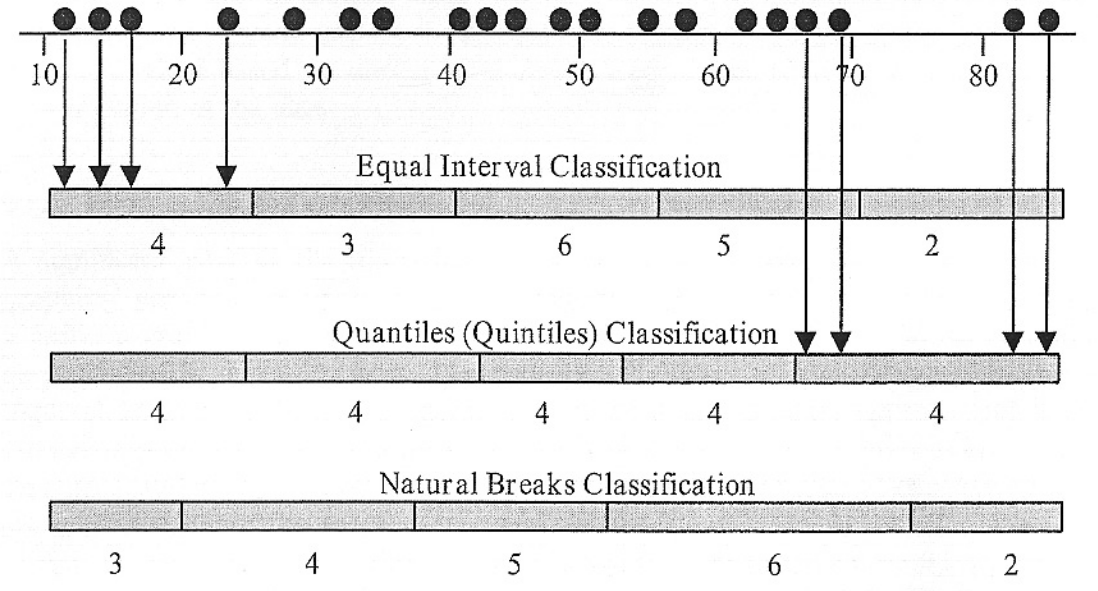
\includegraphics[height=5cm,keepaspectratio]{images/choropleth/classification.png}
\caption[
    Data classification techniques \iacite{McMaster2010}.
]{Data classification techniques}
\label{fig:choropleth-classification}
\end{figure}

\begin{itemize}

\item \textbf{Equal interval classification} assumes equal range between the class breaks. With the mentioned example, class one would include values from 10 to 25, class two would include values from 25 to 40, and so forth \iacite{McMaster2010}.

\item \textbf{Quantiles classification} needs to know the amount of items in a dataset in addition to the amount of desired classes. Consider 100 observations in a dataset and five desired classes. Thus, 20 observations will be placed in each class. These 20 observations can be thought of as data values. Putting this amount of data values in five different classes results in 4 data values per class. Now it is only needed to go through the whole dataset and put the first to the fourth item in the first class, the fifth to the ninth item in the second class, and so forth \iacite{McMaster2010}.

\item \textbf{Natural breaks classification} follows the idea of minimizing the internal variation of the dataset, while maximizing the variation among the classes. The user needs to choose significant gaps in the dataset, according to the number of desired classes \iacite{McMaster2010}.

\end{itemize}

In order to create meaninful choropleth maps, some design principles need to be considered:

\begin{itemize}

\item The visual channel this type of mapping is based on should always be a sequential or diverging color scheme for continuous data, depending on wheter there is a meaningful zero point or not. Figure \ref{fig:colorbrewer} on page \pageref{fig:colorbrewer} shows three different categories of color scales. The reason why choropleth maps should only use diverging or sequential sacles is the perception. These two types are always preceived as ordered. Due to their brightness and saturation, they can be ordered from low to high or vice versa, whereas qualitative scales are perceptually nonlinear. Those scales are best used for categorical data.

\item Choropleth maps are commonly used with data representing derived quantities. Examples of derived quantities are density, average, rate and percentage. If this type of map is not used with such data, it has to be read with caution. Aggregated data e.g. crimes committed or amount of orders can also be used, if the areal bias is taken into consideration when interpreting the map.

\item A choropleth map without a legend is not negotiable, according to \citeauthor{Dent2008}. All colors on the map represent a specific value or class, which is defined and explained in the legend. All classifications would be pointless without a map legend \iacite{Dent2008}.

\end{itemize}

\begin{figure}[!htb]
\centering
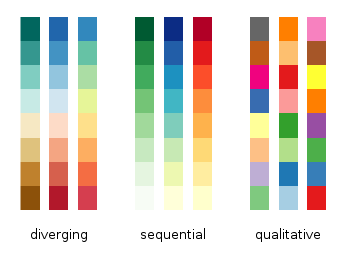
\includegraphics[height=5cm,keepaspectratio]{images/choropleth/color-scales.png}
\caption[
    Three different categories of color scales, Urldate: 07.2016 \newline
    \small\texttt{\url{http://www.gnuplotting.org/figs/colorbrewer.png}}
]{Three different categories of color scales.}
\label{fig:colorbrewer}
\end{figure}

Until now, only so called classed choropleth maps were decribed. Unclassed choropleth maps follow the idea of "letting the data speak for itself". This specific type of a choropleth map assigns a unique color to each unique data value without previous classification. They also make use of a continuous color scale. The major difference to classed ones is best described with an example: consider a dataset consisting of unemployment rates for each state in the united states. If there is a big numerical gap between the second and third highest unemployment rate for two states, their corresponding color would also have a significant jump. Thus the data is placed proportionally along the color scale. Figure \ref{fig:classed-unclassed-choropleth} on page \pageref{fig:classed-unclassed-choropleth} features an unclassed and classed choropleth map.

\begin{figure}[!htb]
  \captionsetup[subfigure]{justification=centering}
  \centering
  \begin{subfigure}[b]{0.4\textwidth}
    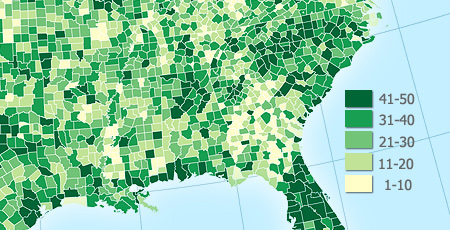
\includegraphics[width=\textwidth]{images/choropleth/classed.jpg}
    \caption{Classed choropleth map.}
  \end{subfigure}
  \hfill
  \begin{subfigure}[b]{0.4\textwidth}
    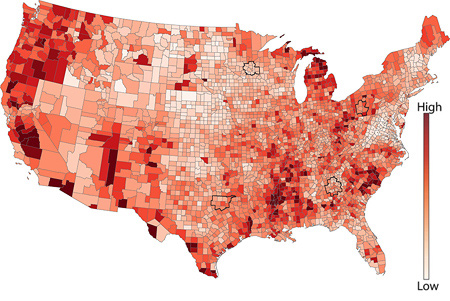
\includegraphics[width=\textwidth]{images/choropleth/unclassed.jpg}
    \caption{Unclassed choropleth map.}
  \end{subfigure}
  \caption[
    Comparison of an unclassed and classed choropleth map, Urldate: 07.2016 \newline
    \small\texttt{\url{http://indiemapper.com/app/learnmore.php?l=choropleth}}
  ]{
    Comparison of an unclassed and classed choropleth map.
  }
  \label{fig:classed-unclassed-choropleth}
\end{figure}

The main objective of choropleth maps is to depict the geographic distribution of the data magnitudes. Ideally the choice of fill will communicate the range from low data magnitudes to high magnitudes through an obvious change from light to dark. If an overall geographic pattern should be shown in the map, an unclassed choropleth map is the way to go. If that is not the case and locations should be comparable against each other, classed choropleth maps should be used.



\label{s:choropleth}

\subparagraph{Cartogram}
From an abstract point of view, a cartogram can be considered a special case of proportional symbol mapping. Instead of a symbol being scaled proportionally to a data magnitute, a cartogram scales its geographic areas. Thus a cartogram includes intentional distortion proportional to the value of an attribute. This also is the reason why some cartograms appear very similar to a map and some have very little sibilance to any kind of map. \citeauthor{Tyner2010} defines a cartogram as a geographic representation where size or distance is scaled to a variable other than earth size or distance units \iacite{Tyner2010}.
There are several types of cartograms. The most commonly seen are value-by-area cartograms. This kind of type is distinguished by the proportional size of enumeration units according to a value. Another type called distance or linear cartogram uses a time scale instead of a distance scale. Value-by-area cartograms are furthermore divided into three types:
\begin{enumerate*}
\item Contiguous,
\item Noncontiguous and
\item different variations of cartograms \iacite{Tyner2010}.
\end{enumerate*}

\begin{enumerate}

\ditem{Contiguous cartograms} \hfill \\
Borders between enumeration units are maintained as much as possible, although shapes are distorted. \citeauthor{Tyner2010} states, that a contiguous cartogram approximating shape with straight line segments is the least confusing one to the reader. Shape is the essential factor for cartograms to preserve information. If individual states cannot be recognized and compared with a conventional map, then a cartogram can have no effect \iacite{Tyner2010}.

\ditem{Noncontiguous cartograms} \hfill \\
Enumeration units are meaningful for this type of cartogram and they show shapes correctly. They either enlarge or reduce the units size according to the variable being mapped. Thus, enumeration units in a noncontiguous cartogram do not touch and are seperated by empty space \iacite{Tyner2010}.

\ditem{Variations} \hfill \\
A dorling cartogram replaces the enumeration units with uniform abstract shapes, normally circles. It tries to place the shapes non-overlapping, whereas maintaining orignial shape or borders not needed. In order to achieve this, the units are moved from their original location. One method of placing the shapes is, to use some kind of collision detection and try to place them as close to their centroid as possible. The demers cartogram is closely related to the dorling cartogram. The only difference is the type of the shape. It uses a square to represent enumeration areas, which gives the advantage of permitting greater contiguity than circles \iacite{Tyner2010}.

\end{enumerate}

A cartogram in general has two major weaknesses:
\begin{enumerate}
\item It distorts geography and therefore standard measurements, e.g. distance among places, are not accurate anymore.
\item Without having the actual geographic shape of the map in mind, it is hard to interpret the cartogram correctly, because the sizes of shapes cannot be related to the enumeration areas anymore.
\end{enumerate}

However, despite their weaknesses, they also have a strong visual impact and therefore attract reader attention. This is definitly an advantage, because it allows for a stronger impression of relative values compared to choropleth or dot density maps. On those type of maps, a high population in a small state is barely noticeable compared to a value-by-area cartogram.
Another minor advantage of a cartogram is its flexibility in data. There is no generalization of data and therefore no loss of detail through it, as this would be the case in classification for choropleth maps \iacite{Tyner2010}.


\paragraph{Multivariate Thematic Map Types}
Multivariate maps are dependent on multiple variables. This section will only give an overview of bivariate maps for the sake of convenience of this type and will not explain them in detail. Some of these maps can be used univariate and multivariate and therefore are not discussed again, if they are alreay explained in detail in chapter \ref{s:univariate-maps} on page \pageref{s:univariate-maps}. However, the needed information to understand limitations and concerns are still added.

\subparagraph{Bivariate Proportional Symbol Map}
Having the need of mapping multiple phenomena on a proportional symbol map exerts in using multiple visual channels. One channel is already fixed due to the chosen map type of proportional symbols. The second channel used for bivariate proportional symbols could be color. According to the data attributed used, a sequential, diverging or qualitative color scale could be used. Every other aspects of bivariate proportional symbol maps are the same as univariate ones.

\subparagraph{Bivariate Choropleth Map}
Bivariate choropleth maps follow the same concept as univariate choropleth maps (see chapter \ref{s:choropleth} on page \pageref{s:choropleth} for more information), except hey show two phenomenons at once. Therefore two datasets need to be combined to show how much of the first variable and the second variable exist in each enumeration unit. The main concept and design goals aswell as data standardization and classification still apply to the multivariate version. The only adaption pertains to the color scale. Figure \ref{fig:bi-scale} on page \pageref{fig:bi-scale} shows two possible color scales. The main difference between sequential and diverging color scales are already explained in detail and therefore using either a sequential (see figure \ref{fig:bi-seq} on page \pageref{fig:bi-seq}) or diverging (see figure \ref{fig:bi-div} on page \pageref{fig:bi-div}) color scale matrix should be clear.


\begin{figure}[!htb]
  \captionsetup[subfigure]{justification=centering}
  \centering
  \begin{subfigure}[b]{0.4\textwidth}
    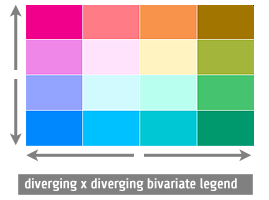
\includegraphics[width=\textwidth]{images/choropleth/divxdiv.png}
    \caption{Diverging x diverging bivariate color scale.}
    \label{fig:bi-div}
  \end{subfigure}
  \hfill
  \begin{subfigure}[b]{0.4\textwidth}
    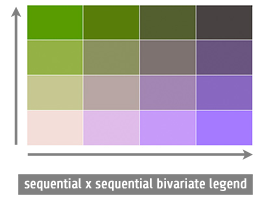
\includegraphics[width=\textwidth]{images/choropleth/seqxseq.png}
    \caption{Sequential x sequential bivariate color scale.}
    \label{fig:bi-seq}
  \end{subfigure}
  \caption[
    Bivariate color scale for choropleth maps, Urldate: 04.2014 \newline
    \small\texttt{\url{https://axismaps.github.io/thematic-cartography/images/seqxseq.png}} \newline
    \small\texttt{\url{https://axismaps.github.io/thematic-cartography/images/divxdiv.png}}
  ]{
    Bivariate color scale for choropleth maps.
  }
  \label{fig:bi-scale}
\end{figure}

\subparagraph{Bivariate Cartogram}
Univariate value-by-area cartograms have the strength of not needing any color. Thus a second theme can be easily added to cartograms e.g. by using color as an additional visual channel.